% Options for packages loaded elsewhere
\PassOptionsToPackage{unicode}{hyperref}
\PassOptionsToPackage{hyphens}{url}
%
\documentclass[
]{book}
\usepackage{lmodern}
\usepackage{amssymb,amsmath}
\usepackage{ifxetex,ifluatex}
\ifnum 0\ifxetex 1\fi\ifluatex 1\fi=0 % if pdftex
  \usepackage[T1]{fontenc}
  \usepackage[utf8]{inputenc}
  \usepackage{textcomp} % provide euro and other symbols
\else % if luatex or xetex
  \usepackage{unicode-math}
  \defaultfontfeatures{Scale=MatchLowercase}
  \defaultfontfeatures[\rmfamily]{Ligatures=TeX,Scale=1}
\fi
% Use upquote if available, for straight quotes in verbatim environments
\IfFileExists{upquote.sty}{\usepackage{upquote}}{}
\IfFileExists{microtype.sty}{% use microtype if available
  \usepackage[]{microtype}
  \UseMicrotypeSet[protrusion]{basicmath} % disable protrusion for tt fonts
}{}
\makeatletter
\@ifundefined{KOMAClassName}{% if non-KOMA class
  \IfFileExists{parskip.sty}{%
    \usepackage{parskip}
  }{% else
    \setlength{\parindent}{0pt}
    \setlength{\parskip}{6pt plus 2pt minus 1pt}}
}{% if KOMA class
  \KOMAoptions{parskip=half}}
\makeatother
\usepackage{xcolor}
\IfFileExists{xurl.sty}{\usepackage{xurl}}{} % add URL line breaks if available
\IfFileExists{bookmark.sty}{\usepackage{bookmark}}{\usepackage{hyperref}}
\hypersetup{
  pdftitle={Style Guide for Loss Data Analytics},
  pdfauthor={An open text authored by the Actuarial Community},
  hidelinks,
  pdfcreator={LaTeX via pandoc}}
\urlstyle{same} % disable monospaced font for URLs
\usepackage{longtable,booktabs}
% Correct order of tables after \paragraph or \subparagraph
\usepackage{etoolbox}
\makeatletter
\patchcmd\longtable{\par}{\if@noskipsec\mbox{}\fi\par}{}{}
\makeatother
% Allow footnotes in longtable head/foot
\IfFileExists{footnotehyper.sty}{\usepackage{footnotehyper}}{\usepackage{footnote}}
\makesavenoteenv{longtable}
\usepackage{graphicx,grffile}
\makeatletter
\def\maxwidth{\ifdim\Gin@nat@width>\linewidth\linewidth\else\Gin@nat@width\fi}
\def\maxheight{\ifdim\Gin@nat@height>\textheight\textheight\else\Gin@nat@height\fi}
\makeatother
% Scale images if necessary, so that they will not overflow the page
% margins by default, and it is still possible to overwrite the defaults
% using explicit options in \includegraphics[width, height, ...]{}
\setkeys{Gin}{width=\maxwidth,height=\maxheight,keepaspectratio}
% Set default figure placement to htbp
\makeatletter
\def\fps@figure{htbp}
\makeatother
\setlength{\emergencystretch}{3em} % prevent overfull lines
\providecommand{\tightlist}{%
  \setlength{\itemsep}{0pt}\setlength{\parskip}{0pt}}
\setcounter{secnumdepth}{5}
\usepackage{booktabs}
\usepackage{hyperref}
\hypersetup{colorlinks,%
citecolor=blue,%
linkcolor=blue,%
urlcolor=blue,%
pdftex}
\usepackage{booktabs}
\usepackage{longtable}
\usepackage{array}
\usepackage{multirow}
\usepackage{wrapfig}
\usepackage{float}
\usepackage{colortbl}
\usepackage{pdflscape}
\usepackage{tabu}
\usepackage{threeparttable}
\usepackage{threeparttablex}
\usepackage[normalem]{ulem}
\usepackage{makecell}
\usepackage{xcolor}
\usepackage[]{natbib}
\bibliographystyle{apalike}

\title{Style Guide for Loss Data Analytics}
\author{An open text authored by the Actuarial Community}
\date{2020-08-13}

\begin{document}
\maketitle

{
\setcounter{tocdepth}{1}
\tableofcontents
}
\hypertarget{preface}{%
\chapter*{Preface}\label{preface}}
\addcontentsline{toc}{chapter}{Preface}

It is important for chapters in the \emph{Open Actuarial Textbooks} project to have a consistent look and feel. The \emph{Style Guide for Loss Data Analytics} aims to assist contributors in developing chapters consistently throughout the \emph{Loss Data Analytics} book.

This guide is set up as sample chapters containing

\begin{itemize}
\tightlist
\item
  information regarding suitable content for a chapter,
\item
  methods to implement chapter elements and
\item
  conventions for consistent notation.
\end{itemize}

\hypertarget{chapter-structure}{%
\chapter{Chapter Structure}\label{chapter-structure}}

\begin{center}\rule{0.5\linewidth}{0.5pt}\end{center}

In this chapter, you learn how to:

\begin{itemize}
\tightlist
\item
  Determine what and what not to include in a chapter
\item
  Include technical supplements as needed
\item
  Assess types of exercises and book resources that are appropriate for a chapter
\end{itemize}

\begin{center}\rule{0.5\linewidth}{0.5pt}\end{center}

\hypertarget{chapter-preview-and-learning-objectives}{%
\section{Chapter Preview and Learning Objectives}\label{chapter-preview-and-learning-objectives}}

\begin{itemize}
\item
  \emph{Chapter Preview}. Begin with a chapter preview to set the stage of the chapter.
\item
  \emph{Learning Objectives}. At the beginning of each chapter and section, describe in a few bullet points what the reader can expect to learn.
\end{itemize}

\hypertarget{main-body}{%
\section{Main Body}\label{main-body}}

Split the chapter into 4-7 sections; within each section, introduce 0-5 subsections. Do not develop a deeper hierarchy (e.g., a ``sub-subsection''). Use nonlinear aspects of the web. For example, detailed mathematical developments can go into a technical appendix or are simply hidden (using javascript ``hide/show'' tools) unless the viewer really wants to see the details. Case studies and historical references can be included in ``side-bars,'' a supporting webpage. For the main body of the chapter, think about ``25 pages'' in length (whatever that means\ldots.).

\hypertarget{what-to-include}{%
\subsection{What to Include}\label{what-to-include}}

\begin{itemize}
\item
  Within the chapter, use boxed and numbered lists of procedures for easy reference.
\item
  It is certainly okay (and expected) to use mathematical notation although please adhere to the conventions described in Section \ref{S:NotationConvention}. Each chapter should have examples interwoven within theory, allowing readers to see the development of the theory along with the importance of the applications.
\item
  Distinguish between an \emph{``Example''} and a \emph{``Special Case''}. The former shows how to relate the mathematics to a practical situation likely to be encountered by a practicing actuary. The latter looks at a subset of a general (usually) mathematical result. A few special cases are certainly acceptable but we want to focus on developing examples.
\item
  Think of graphical ways to visualize/summarize relationships that you want to emphasize.
\item
  Begin each section with a short bullet list describing the learning objectives of that section. Finish each section with a short quiz on these learning objectives. As of this writing (July 2018), quizzes are multiple-choice.
\item
  Include short exercises/examples/special cases that can be readily solved by the viewer (with solutions using ``hide/show'' features) within the main body. These serve to reinforce concepts and provide benchmarks for understanding.
\end{itemize}

\hypertarget{what-not-to-include}{%
\subsection{What Not to Include}\label{what-not-to-include}}

\begin{itemize}
\item
  Do not include development of equations/formulas in the main body of the text. The main body of the text will be devoted to presenting results, providing context and intuition as to the importance of the results.
\item
  Do not include references to the literature. This will appear in the last section on ``Further Reading and References.''
\item
  Do not include graphs whose information could easily be summarized by a table.
\end{itemize}

\hypertarget{technical-supplements}{%
\section{Technical Supplements}\label{technical-supplements}}

We want our viewers to understand the underpinnings of the theory (the old analogy of ``what is going on under the hood to see how the engine works'' - no black boxes.) So, there will be occasions when you feel like a short development or ``proof''; is reasonable. Put this in an appendix. Technical supplements should develop the theory in a step-by-step fashion, building on each concept in a crisp, mathematical fashion.

\hypertarget{S:further-reading-and-resources}{%
\section{Contributors and Further Resources}\label{S:further-reading-and-resources}}

\hypertarget{contributors}{%
\subsection{Contributors}\label{contributors}}

Make sure that contributors are listed at the end of the chapter. The following provides an example.

\begin{verbatim}
####Contributors {-}

- Edward W. (Jed) Frees, University of Wisconsin-Madison, 
is the principal author of the initital version of this chapter. 
Email: jfrees@bus.wisc.edu for chapter comments and 
suggested improvements. Helpful improvements provided by
Alyaa Nuval Binti Othman and Aisha Nuval Binti Othman.
\end{verbatim}

\hypertarget{further-reading-and-references}{%
\subsection{Further Reading and References}\label{further-reading-and-references}}

Do not finish with a ``preview of upcoming chapter''; finish instead with a ``Further Reading and References.'' This consists of a series of references with one or two lines of annotation for each reference that the interested reader could follow up on (self-citations are okay!). Historical developments are particularly nice in this section.

\hypertarget{S:Interactive}{%
\chapter{Interactive Book Features}\label{S:Interactive}}

An advantage of publishing on the web is that we can produce an online version that contains many interactive objects such as quizzes, computer demonstrations, interactive graphs, video, and the like, to promote \textbf{deeper learning}.

We want viewers to interact with the book; it is \textbf{not} written to accommodate the ``armchair reader,'' that is, one who passively reads and does not get involved by attempting the exercises in the text. Consider an analogy to sports; there is a great deal that you can learn about the game just by watching. However, if you want to sharpen your skills, then you have to go out and play the game.

\#\#Examples and Exercises

Even for traditional offline (pdf) version of the book, we include problems that allow readers to develop their learning.

Each chapter contains several ``Examples'' or ``Exercises'' - these are focused problems that generally ask the reader to do a calculation or provide an interpretation of a statistical issue. We call them ``examples'' when they appear in the main body of the text and ``exercises'' when they appear at the end of the chapter. The need for hand calculations has been advocated by Khamis (1991)\footnote{``Manual Computations---A Tool for Reinforcing Concepts and Techniques,'' H. J. Khamis, Pages 294-299, \emph{The American Statistician}, Volume 45, 1991 - Issue 4}. Many teachers have found it useful to practice the mechanics in order to provide a solid foundation. With this foundation, we can get on to the real business; interpreting data using statistical principles.

We anticipate that substantial exercise banks will be built over time by users, professional associations, and those with commercial interests. When developing the chapter foundations, think about the following types of problems.

\begin{itemize}
\tightlist
\item
  \textbf{Hand Calculation.} These are problems that can be solved without the use of a computer. They typically reinforce a statistical or actuarial concept as well as highlight an issue that might be encountered in practice. For this book, these problems often involve algebraic and calculus manipulations. When writing these types of problems, readers are more motivated if they understand \emph{why} the problem is important. What actuarial issue is being addressed? What statistical concept is being practiced? Often, a simple line or two prefacing a problem can help substantially in this regard.
\item
  \textbf{Software.} These are problems that ask the reader to work with \texttt{R} software, such as calculating a function or reproducing a graph.
\item
  \textbf{Data.} These are problems that ask the reader to work with data. The need for working with real data is well documented; for example, see Hogg (1972), Moore and Roberts (1989) or Singer and Willett (1990). By providing detailed guided tutorials that work with theory and data, we teach our students the essence of \emph{Loss Data Analytics}. Of course, there are some important disadvantages to working with real data. Data sets can quickly become outdated. Further, the ideal data set to illustrate a specific statistical issue is difficult to find. Data exercises are complex and can span several chapter sections as well as chapters.
\end{itemize}

Examples and exercises are designed so that they illustrate a general analytics/statistical concept; they have the additional advantage in that they are often based on actuarial professional examinations and so provide readers with training for these assessment frameworks. Notably, \emph{in the online version of the book, the solutions to the examples and exercises are hidden to encourage readers to actively solve (or at least consider) prior to revealing a solution.}

\#\#Statistical Code

However, the limitation of exercise and examples done by hand is that they give \textbf{little insight} as to how the general analytics/statistical concepts can be used in applications or why more extensive treatments beyond the foundations would be needed. To address these limitations, throughout we include illustrate statistical code with sample (but real) datasets. The statistical language used throughout is \texttt{R}. For two reasons, the \texttt{R} code is hidden in the online version but can be interactively revealed but clicking a button.

\begin{itemize}
\tightlist
\item
  First, we want to focus on the analytics/statistical concepts and do not wish for readers to be distracted by software code that emphasizes implementation, not concepts.
\item
  Second, not all readers will use \texttt{R} (there are many good alternative software programs available) and we want the book to be available to a broad readership.
\end{itemize}

Although we do not focus on developing \texttt{R} tutorials, we will provide guides and links to people who wish to learn \texttt{R}. Our focus is on teaching statistical methods and actuarial issues, not software. Over time, the project may also provide support for users of other software environments, such as Microsoft's Excel or Python.

\#\#Other Interactive Features

A wonderful aspect of an online text is that we can readily incorporate other interactive features. In coming versions of the book, you can expect to see

\begin{itemize}
\tightlist
\item
  a glossary (hover the cursor over a technical word or phrase to reveal a definition),
\item
  links to relevant applications of the basic concept, as well as
\item
  end of the section quizzes that provide ``low-level formative assessments'' so that they reader can gauge his or her understanding of the material.
\end{itemize}

Some of the support material associated with the book also emphasizes interactive aspects. For example, detailed \emph{R code} allows readers to learn complex statistical routines and provides sample code so that users can develop their own libraries of useful routines. Another site will feature \texttt{R-Shiny}, an interactive graphic tool that provides dynamic graphing features. The concept of active learning promotes one of the deeper learning goals set forth by some educational leaders: The ability to learn how to learn independently.

\hypertarget{additional-book-resources-supporting-each-chapter}{%
\section{Additional Book Resources Supporting Each Chapter}\label{additional-book-resources-supporting-each-chapter}}

We are hopeful that there will be several resources support the book that will appear outside of the chapter structure. Although not necessarily interactive, they will help develop users' learning. These include:

\begin{itemize}
\tightlist
\item
  \textbf{Case Studies and Historical Vignettes.} Similar to those appearing within the chapter, include short exercises/examples/special cases that can be readily solved by the viewer. These serve to reinforce concepts and provide benchmarks for understanding. Case studies can be used to emphasize different practices in different countries. Historical vignettes can be interesting in their own right and remind us all of the foundations of our discipline.
\item
  \textbf{Data.} We anticipate developing a library of data sets that can be used by instructors who wish to emphasize different areas of practice.
\item
  \textbf{Technical Supplements, Lists, and Tables.} The roles of technical supplements has already been described and there could be many. As is common in textbooks, we will also provide a place for lists or tables of organized facts for learners.
\end{itemize}

\hypertarget{S:SampleSection}{%
\chapter{\texorpdfstring{Samples of Writing in \texttt{R\ bookdown}}{Samples of Writing in R bookdown}}\label{S:SampleSection}}

\begin{center}\rule{0.5\linewidth}{0.5pt}\end{center}

In this chapter, you learn how to:

\begin{itemize}
\tightlist
\item
  Reference other sections and equations
\item
  Include in-text citation that links to the bibliography
\item
  Include tables and figures not generated by \texttt{R} code
\item
  Include a footnote
\item
  Add tooltip descriptions for technical phrases
\item
  Include chapter examples and R code
\end{itemize}

\begin{center}\rule{0.5\linewidth}{0.5pt}\end{center}

As we expand our contributor and reviewer base, it will be helpful to know more about the conventions used in the series regarding the details of \texttt{R\ markdown} and \texttt{R\ bookdown} used in the series. This chapter summarizes these conventions.

\hypertarget{S:SectionLabels}{%
\section{Section Labels and Learning Objectives}\label{S:SectionLabels}}

The following shows how to code Section titles and refer to them.

\begin{verbatim}
## Section Labels {#S:SectionLabels}
\end{verbatim}

With that reference, one can readily refer to Section \ref{S:SectionLabels} in your text, as follows:

\begin{verbatim}
With that reference, one can readily refer to 
Section \\ref{S:SectionLabels} in your text, as follows:
\end{verbatim}

The following shows how to code learning objectives:

\begin{verbatim}
***
In this chapter, you learn how to:
  
- Reference other sections and equations
- Include in-text citation that links to the bibliography
- Include tables and figures
- Include a footnote

***

\end{verbatim}

\hypertarget{equation-references}{%
\section{Equation References}\label{equation-references}}

Here is an example of a latex equation produced in \texttt{R\ markdown}, with reference number.

\begin{equation}
  x + y = 1  
\label{eq:ExampleEquation}
\end{equation}

You can produce that equation using the following code.

\begin{verbatim}
\begin{equation}
  x + y = 1  
\label{eq:ExampleEquation}
\end{equation}
\end{verbatim}

With this, equation \eqref{eq:ExampleEquation} can be referred to using the following code:

\begin{verbatim}
With this, equation \\eqref{eq:ExampleEquation} can be 
referred to using the following code:
\end{verbatim}

\hypertarget{in-text-citations}{%
\section{In-text Citations}\label{in-text-citations}}

Here is an example of an in-text citation made possible by \texttt{R\ bookdown} \citep{xie2015}. This links to the bibliography where the full referece is displayed. As a convention we use the \emph{APA} style citation.

\begin{verbatim}
Here is an example of an in-text citation made possible by 
`R bookdown` [@xie2015]. This links to the bibliography 
where the full reference is displayed. 
As a convention we use the *APA* style citation.
    
\end{verbatim}

\hypertarget{including-tables}{%
\section{Including Tables}\label{including-tables}}

We want to be able to include Latex tables (for mathematical type), as well as data-drive tables produced by \texttt{R}. In order to do that, we use html syntax in order to reference tables. This means that we have to number the tables by hand. Although a bit painful, it does gives us the flexibility needed.

Start with a Latex generated table.

\textbf{Table 2.1. An Example of Including Tables using Latex in an \texttt{R\ markdown} Document}

\[
\begin{matrix}
    \begin{array}{c|c} \hline
    \text{Policyholder} & \text{Number of claims} \\\hline
    \textbf{X} & 1 \\\hline
    \textbf{Y} & 2 \\\hline
    \end{array}
\end{matrix}
\]

\texttt{R\ markdown} does not have a convention for referencing non-R generated tables. For now, we reference them manually as in refer to \protect\hyperlink{tab:2.1}{Table 2.1}. We do this by manually inserting an html anchor tag.

The following code produces this table.

\begin{verbatim}
<a id=tab:2.1></a> 

[Table 2.1]: \#tab:2.1

##### Table 2.1. An Example of Including Tables using Latex in an `R markdown` Document {-}

$$
\begin{matrix}
    \begin{array}{c|c} \hline
    \text{Policyholder} & \text{Number of claims} \\\hline
    \textbf{X} & 1 \\\hline
    \textbf{Y} & 2 \\\hline
    \end{array}
\end{matrix}
$$
    
\end{verbatim}

For reference, then use

\begin{verbatim}

`R markdown` does not have a convention for referencing 
non-R generated tables. For now, we reference them manually 
as in refer to [Table 2.1].
\end{verbatim}

Now we give a data-driven table generated by \texttt{R} in \protect\hyperlink{tab:2.2}{Table 2.2}.

\textbf{Table 2.2. An Example of Including Tables using \texttt{R} }

\begin{table}[H]
\centering
\resizebox{\linewidth}{!}{
\begin{tabular}{r|r|r|r|r|r}
\hline
Minimum & First Quartile & Median & Mean & Third Quartile & Maximum\\
\hline
167 & 2226 & 4951 & 56332 & 11900 & 12922218\\
\hline
\end{tabular}}
\end{table}

Here is the code to produce this table.

\begin{verbatim}

<a id=tab:2.2></a> 

[Table 2.2]: \#tab:2.2


```r
Insample <- read.csv("Insample.csv", header=T,  
              na.strings=c("."), stringsAsFactors=FALSE)
Insample2010 <- subset(Insample, Year==2010)
InsamplePos2010 <- subset(Insample2010, yAvg>0)
summaryOutput <- t(as.matrix(summary(InsamplePos2010$yAvg)))
colnames(summaryOutput) <- c("Minimum","First Quartile", 
                             "Median", "Mean", "Third Quartile", "Maximum")
kable_styling(knitr::kable(summaryOutput,digits=0, 
                    align = "rrrrrr"), latex_options="scale_down")
```
\end{verbatim}

\hypertarget{including-figures}{%
\section{Including Figures}\label{including-figures}}

\hypertarget{figures-generated-by-r}{%
\subsection{\texorpdfstring{Figures Generated by \texttt{R}}{Figures Generated by R}}\label{figures-generated-by-r}}

Most figures are generated using \texttt{R}. Here is an illustrative figure.

\begin{figure}

{\centering 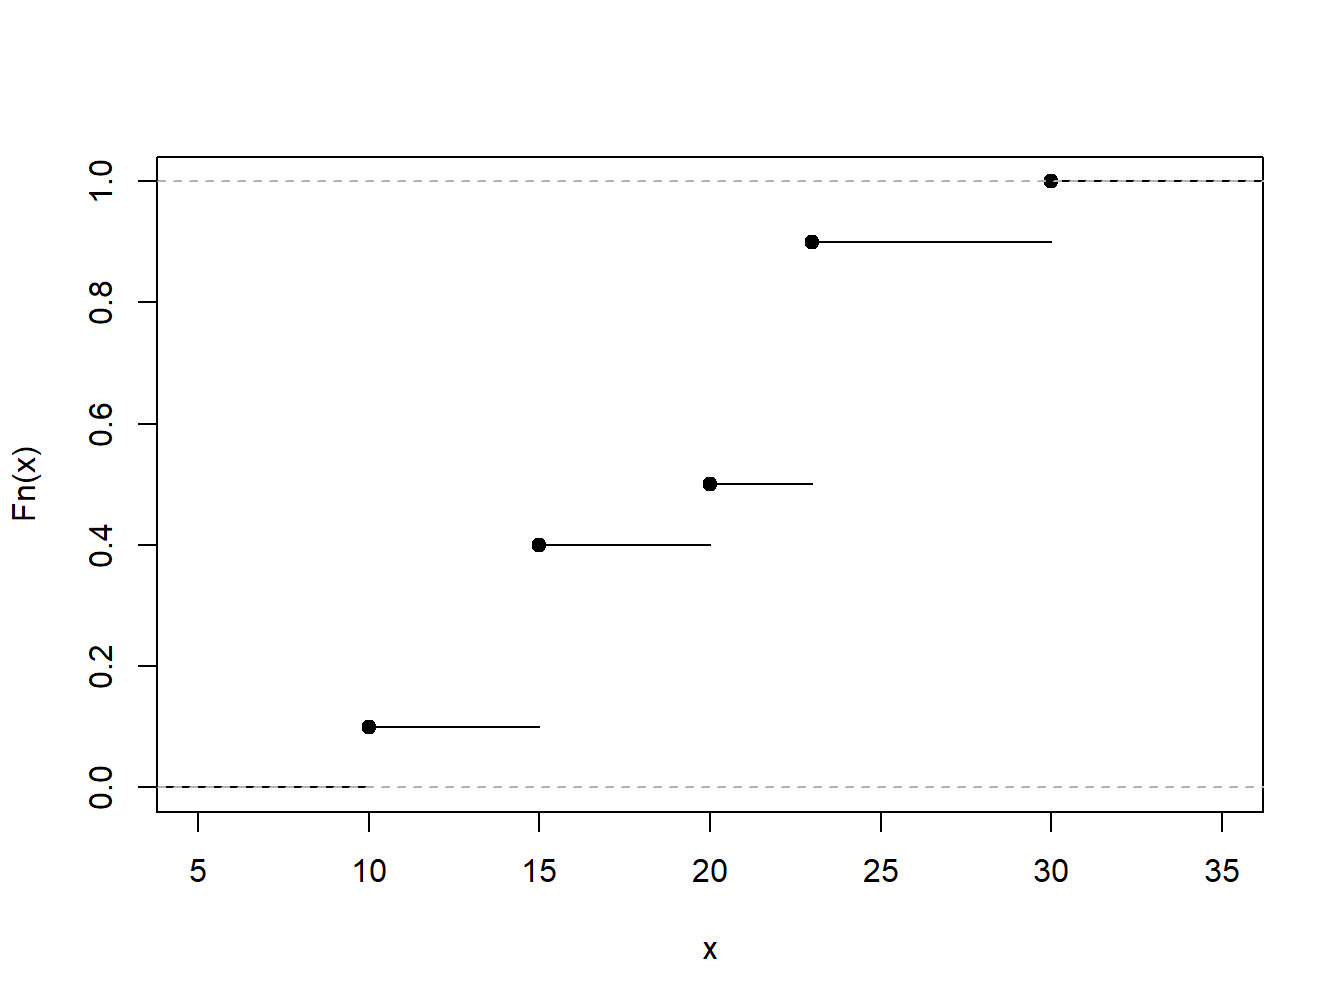
\includegraphics[width=0.6\linewidth]{Style-Guide-for-LDA_files/figure-latex/EDFToy-1} 

}

\caption{Empirical Distribution Function of a Toy Example}\label{fig:EDFToy}
\end{figure}

that we refer to as Figure \ref{fig:EDFToy}. Here is the code for producing the figure:

\begin{verbatim}
```{r EDFToy, echo = FALSE, 
   fig.cap = 'Empirical Distribution Function of a Toy Example',
   out.width = '60%', fig.asp = 0.75, fig.align = 'center'}
xExample <- c(10,rep(15,3),20,rep(23,4),30)
PercentilesxExample <- ecdf(xExample)
plot(PercentilesxExample, main = "", xlab = "x")
```
\end{verbatim}

Here is is the code for referencing the Figure \ref{fig:EDFToy}:

\begin{verbatim}
Here is is the code for referencing the Figure \\ref{fig:EDFToy}:
    
\end{verbatim}

\hypertarget{figures-not-generated-by-r}{%
\subsection{\texorpdfstring{Figures Not Generated by \texttt{R}}{Figures Not Generated by R}}\label{figures-not-generated-by-r}}

For figures, we store the figures as png or jpeg files in a separate folder called ``Figures''. Then we use \texttt{R} code to call those figures for display so that we can reference them.

Here is such a figure:

\begin{figure}

{\centering \includegraphics[width=0.05\linewidth]{Figures/RStudio-Ball} 

}

\caption{An example of including figures in an R Markdown document}\label{fig:ExampleFigure}
\end{figure}

And here is the code that generates the figure:

\begin{verbatim}
"three backticks"{r, ExampleFigure, fig.cap = 'An example 
of including figures in an R Markdown document', 
out.width = '5%', fig.align = 'center', echo = FALSE}
knitr::include_graphics("Figures/RStudio-Ball.png")
"three backticks"
\end{verbatim}

Here is is the code for referencing the Figure \ref{fig:ExampleFigure}:

\begin{verbatim}
Here is is the code for referencing the Figure \\ref{fig:ExampleFigure}:
    
\end{verbatim}

\hypertarget{including-footnotes}{%
\section{Including Footnotes}\label{including-footnotes}}

Try to minimize the use of footnotes. But, if you need them, here is how you can include a footnote \footnote{the footnote displays at the end of the chapter}.

\begin{verbatim}
Here is how you can include a footnote [^1].
    
[^1]: the footnote displays at the end of the chapter
    
\end{verbatim}

\hypertarget{defining-glossary-terms}{%
\section{Defining Glossary Terms}\label{defining-glossary-terms}}

Use the \texttt{Gloss(term)} function to include a tooltip for technical phrases. \texttt{Gloss(term)} looks up the definition in \texttt{GlossFct.csv}. Accordingly, you can add new glossary terms for your chapter in the \texttt{csv} file.

Here is how you add a tooltip:

We can use the same \texttt{Gloss(term)} function to include tooltips for acronyms (e.g.~iid) as listed in Section \ref{S:Abbreviations}.

\hypertarget{glossary-conventions}{%
\subsection{Glossary Conventions}\label{glossary-conventions}}

\begin{itemize}
\tightlist
\item
  Include tooltip for a term only once in a chapter.
\item
  Include tooltip when the term is defined. (e.g.~``Frequency is \ldots{}'')
\item
  If term is not explicitly defined, include tooltip at the term's first occurence in the chapter.
\item
  Only include tooltip in the Chapter Preview or in examples if the term is not defined elsewhere in the chapter.
\end{itemize}

\hypertarget{glossary-terms-with-multiple-definitions}{%
\subsection{Glossary Terms with Multiple Definitions}\label{glossary-terms-with-multiple-definitions}}

A term may carry multiple definitions across different sections. In this case, use \texttt{Gloss(term,\ section)}:

\hypertarget{including-chapter-examples-and-r-code}{%
\section{Including Chapter Examples and R Code}\label{including-chapter-examples-and-r-code}}

As described in Section \ref{S:Interactive}, chapter examples and R code allow readers to interact with the online version of the book.

Here is how to add a chapter example:

Similarly, you can add statistical code:

and also proof theory:

\texttt{HideExample}, \texttt{HideRCode}, and \texttt{HideProofTheory} are R functions that can hide these interactive features in the offline (pdf) version of the book. All you need to do is change \texttt{eval\ =\ TRUE} in \texttt{PdfOutput.Rmd}.

\hypertarget{S:Links}{%
\section{Useful Links}\label{S:Links}}

Naturally, you will want to learn more about coding in \texttt{R\ markdown}, \texttt{R\ bookdown} and so forth. The following provide some useful links for taking the next step.

\begin{itemize}
\item
  For an \texttt{R\ markdown} guide refer \url{https://rmarkdown.rstudio.com/authoring_pandoc_markdown.html}.
\item
  For a \texttt{R\ bookdown} guide, see \url{https://bookdown.org/yihui/bookdown/}.
\item
  For best practices in coding \texttt{R}, we suggest
  \url{http://r-pkgs.had.co.nz/style.html}.
\item
  See also our online actuarial text resources at
  \url{https://sites.google.com/a/wisc.edu/loss-data-analytics/online-actuarial-text-resources}.
\end{itemize}

\hypertarget{setting-up-a-glossary}{%
\chapter{Setting up a Glossary}\label{setting-up-a-glossary}}

\begin{center}\rule{0.5\linewidth}{0.5pt}\end{center}

In this chapter, you learn how to:

\begin{itemize}
\tightlist
\item
  Setup csv files for a glossary
\item
  List terms and definitions by chapter
\item
  List terms by the chapter in which they are first defined
\item
  Use GitHub to store the project, make changes, seek feedback and facilitate collaboration
\end{itemize}

\begin{center}\rule{0.5\linewidth}{0.5pt}\end{center}

A glossary can serve as a quick reference when the reader needs to recall a term's definition or location within a book. This chapter can serve as a guide to setup a glossary in the \texttt{R\ Bookdown} environment. Please refer \href{https://bookdown.org/yihui/bookdown/get-started.html}{here} for a refresher on \texttt{R\ Bookdown} if necessary.

\hypertarget{csv-file-setup}{%
\section{csv File Setup}\label{csv-file-setup}}

The following outlines how we currently store our glossary:

\begin{enumerate}
\def\labelenumi{\arabic{enumi}.}
\tightlist
\item
  Setup an excel file with 3 columns: Term, Definition, Chapter first defined.
\item
  We suggest using one excel file for all chapters for easy reference and sharing. However, you will have to save each chapter separately. Alternatively, you may use one excel file per chapter instead of having one central file then separating it.
\item
  Save the Excel file as a csv file.
\item
  Please note that if you make changes, do so in the Excel file not the csv file.
\end{enumerate}

\hypertarget{terms-and-definitions-by-chapter}{%
\section{Terms and Definitions by Chapter}\label{terms-and-definitions-by-chapter}}

This section describes how to create a list of important terms and their definitions listed according to the chapters in which they are found.

We use an example from the glossary of Loss Data Analytics. First we display the list of terms and definitions for Chapter 1 of the book followed by the code used to generate it.

\hypertarget{chapter-1-introduction-to-loss-data-analytics}{%
\subsection{Chapter 1 Introduction to Loss Data Analytics}\label{chapter-1-introduction-to-loss-data-analytics}}

\begin{longtable}[]{@{}cc@{}}
\toprule
\begin{minipage}[b]{0.39\columnwidth}\centering
Term\strut
\end{minipage} & \begin{minipage}[b]{0.43\columnwidth}\centering
Definition\strut
\end{minipage}\tabularnewline
\midrule
\endhead
\begin{minipage}[t]{0.39\columnwidth}\centering
loss adjustment expenses\strut
\end{minipage} & \begin{minipage}[t]{0.43\columnwidth}\centering
Loss adjustment expenses are
costs to the insurer that are
directly attributable to
settling a claims. For
example, the cost of an
adjuster is someone who assess
the claim cost or a lawyer who
becomes involve in settling an
insurer's legal obligation on
a claim\strut
\end{minipage}\tabularnewline
\begin{minipage}[t]{0.39\columnwidth}\centering
unallocated loss adjustment
expenses\strut
\end{minipage} & \begin{minipage}[t]{0.43\columnwidth}\centering
Unallocated loss adjustment
expenses are costs that can
only be indirectly attributed
to claim settlement; for
example, the cost of an office
to support claims staff\strut
\end{minipage}\tabularnewline
\begin{minipage}[t]{0.39\columnwidth}\centering
allocated loss adjustment
expenses\strut
\end{minipage} & \begin{minipage}[t]{0.43\columnwidth}\centering
Allocated loss adjustment
expenses, sometimes known by
the acronym ALEA, are costs
that can be directly
attributed to settling a
claim; for example, the cost
of an adjuster\strut
\end{minipage}\tabularnewline
\begin{minipage}[t]{0.39\columnwidth}\centering
indemnification\strut
\end{minipage} & \begin{minipage}[t]{0.43\columnwidth}\centering
Indemnification is the
compensation provided by the
insurer.\strut
\end{minipage}\tabularnewline
\begin{minipage}[t]{0.39\columnwidth}\centering
insurance claim\strut
\end{minipage} & \begin{minipage}[t]{0.43\columnwidth}\centering
An insurance claim is the
compensation provided by the
insurer for incurred hurt,
loss, or damage that is
covered by the policy.\strut
\end{minipage}\tabularnewline
\begin{minipage}[t]{0.39\columnwidth}\centering
loss amount\strut
\end{minipage} & \begin{minipage}[t]{0.43\columnwidth}\centering
The loss amount is the size of
the loss incurred by the
policyholder for incurred
hurt, loss, or damage that is
covered by the policy.\strut
\end{minipage}\tabularnewline
\begin{minipage}[t]{0.39\columnwidth}\centering
analytics\strut
\end{minipage} & \begin{minipage}[t]{0.43\columnwidth}\centering
Analytics is the process of
using data to make decisions.\strut
\end{minipage}\tabularnewline
\begin{minipage}[t]{0.39\columnwidth}\centering
renters insurance\strut
\end{minipage} & \begin{minipage}[t]{0.43\columnwidth}\centering
Renters insurance is an
insurance policy that covers
the contents of an apartment
or house that you are renting.\strut
\end{minipage}\tabularnewline
\begin{minipage}[t]{0.39\columnwidth}\centering
homeowners insurance\strut
\end{minipage} & \begin{minipage}[t]{0.43\columnwidth}\centering
Homeowners insurance is an
insurance policy that covers
the contents and property of a
building that is owned by you
or a friend.\strut
\end{minipage}\tabularnewline
\begin{minipage}[t]{0.39\columnwidth}\centering
automobile insurance\strut
\end{minipage} & \begin{minipage}[t]{0.43\columnwidth}\centering
An insurance policy that
covers damage to your vehicle,
damage to other vehicles in
the accident, as well as
medical expenses of those
injured in the accident.\strut
\end{minipage}\tabularnewline
\begin{minipage}[t]{0.39\columnwidth}\centering
property insurance\strut
\end{minipage} & \begin{minipage}[t]{0.43\columnwidth}\centering
Property insurance is a policy
that protects the insured
against loss or damage to real
or personal property. The
cause of loss might be fire,
lightening, business
interruption, loss of rents,
glass breakage, tornado,
windstorm, hail, water damage,
explosion, riot, civil
commotion, rain, or damage
from aircraft or vehicles.\strut
\end{minipage}\tabularnewline
\begin{minipage}[t]{0.39\columnwidth}\centering
nonlife insurance\strut
\end{minipage} & \begin{minipage}[t]{0.43\columnwidth}\centering
Nonlife insurance is any type
of insurance where payments
are not based on the death (or
survivorship) of a named
insured. Examples include
automobile, homeowners, and so
on. Also known as property and
casualty or general insurance.\strut
\end{minipage}\tabularnewline
\begin{minipage}[t]{0.39\columnwidth}\centering
casualty insurance\strut
\end{minipage} & \begin{minipage}[t]{0.43\columnwidth}\centering
Causalty insurance is a form
of liability insurance
providing coverage for
negligent acts and omissions.
Examples include workers
compensation, errors and
omissions, fidelity, crime,
glass, boiler, and various
malpractice coverages.\strut
\end{minipage}\tabularnewline
\begin{minipage}[t]{0.39\columnwidth}\centering
valuation date\strut
\end{minipage} & \begin{minipage}[t]{0.43\columnwidth}\centering
A valuation date is the date
at which a company summarizes
its financial position,
typically quarterly or
annually.\strut
\end{minipage}\tabularnewline
\begin{minipage}[t]{0.39\columnwidth}\centering
underwriting\strut
\end{minipage} & \begin{minipage}[t]{0.43\columnwidth}\centering
Underwriting is the process
where the company makes a
decision as to whether or not
to take on a risk.\strut
\end{minipage}\tabularnewline
\begin{minipage}[t]{0.39\columnwidth}\centering
ratemaking\strut
\end{minipage} & \begin{minipage}[t]{0.43\columnwidth}\centering
\strut
\end{minipage}\tabularnewline
\begin{minipage}[t]{0.39\columnwidth}\centering
reinsurer\strut
\end{minipage} & \begin{minipage}[t]{0.43\columnwidth}\centering
A reinsurer is an insurance
company that offers insurance
to an insurer.\strut
\end{minipage}\tabularnewline
\begin{minipage}[t]{0.39\columnwidth}\centering
loss reserve\strut
\end{minipage} & \begin{minipage}[t]{0.43\columnwidth}\centering
A loss reserve is an estimate
of liability indicating the
amount the insurer expects to
pay for claims that have not
yet been realized. This
includes losses incurred but
not yet reported (IBNR) and
those claims that have been
reported claims that haven't
been paid (known by the
acronym RBNS for reported but
not settled).\strut
\end{minipage}\tabularnewline
\begin{minipage}[t]{0.39\columnwidth}\centering
technical provisions\strut
\end{minipage} & \begin{minipage}[t]{0.43\columnwidth}\centering
Technical provisions is
another name for loss
reserves.\strut
\end{minipage}\tabularnewline
\begin{minipage}[t]{0.39\columnwidth}\centering
experience rating\strut
\end{minipage} & \begin{minipage}[t]{0.43\columnwidth}\centering
\strut
\end{minipage}\tabularnewline
\begin{minipage}[t]{0.39\columnwidth}\centering
merit rating\strut
\end{minipage} & \begin{minipage}[t]{0.43\columnwidth}\centering
\strut
\end{minipage}\tabularnewline
\begin{minipage}[t]{0.39\columnwidth}\centering
risk classification\strut
\end{minipage} & \begin{minipage}[t]{0.43\columnwidth}\centering
Risk classification is the
process of grouping
policyholders into categories,
or classes, where each insured
in the class has a risk
profile that is similar to
others in the class.\strut
\end{minipage}\tabularnewline
\begin{minipage}[t]{0.39\columnwidth}\centering
cream skimming\strut
\end{minipage} & \begin{minipage}[t]{0.43\columnwidth}\centering
\strut
\end{minipage}\tabularnewline
\begin{minipage}[t]{0.39\columnwidth}\centering
claims triage\strut
\end{minipage} & \begin{minipage}[t]{0.43\columnwidth}\centering
\strut
\end{minipage}\tabularnewline
\begin{minipage}[t]{0.39\columnwidth}\centering
pure premium\strut
\end{minipage} & \begin{minipage}[t]{0.43\columnwidth}\centering
Pure premium is the total
severity divided by the number
of claims. It does not include
insurance company expenses,
premium taxes, contingencies,
nor an allowance for profits.
Also called loss costs. Some
definitions include allocated
loss adjustment expenses
(ALAE).\strut
\end{minipage}\tabularnewline
\begin{minipage}[t]{0.39\columnwidth}\centering
loss cost\strut
\end{minipage} & \begin{minipage}[t]{0.43\columnwidth}\centering
Loss cost is the total
severity divided by the number
of claims. It does not include
insurance company expenses,
premium taxes, contingencies,
nor an allowance for profits.
Also called pure premium. Some
definitions include allocated
loss adjustment expenses
(ALAE).\strut
\end{minipage}\tabularnewline
\begin{minipage}[t]{0.39\columnwidth}\centering
rating variables\strut
\end{minipage} & \begin{minipage}[t]{0.43\columnwidth}\centering
\strut
\end{minipage}\tabularnewline
\begin{minipage}[t]{0.39\columnwidth}\centering
coinsurance\strut
\end{minipage} & \begin{minipage}[t]{0.43\columnwidth}\centering
Coinsurance is an arrangement
whereby the insured and
insurer share the covered
losses. Typically, a
coinsurance parameter
specified means that both
parties receive a proportional
share, e.g., 50\%, of the loss.\strut
\end{minipage}\tabularnewline
\begin{minipage}[t]{0.39\columnwidth}\centering
deductible\strut
\end{minipage} & \begin{minipage}[t]{0.43\columnwidth}\centering
A deductible is a parameter
specified in the contract.
Typically, losses below the
deductible are paid by the
policyholder whereas losses in
excess of the deductible are
the insurer's responsibility
(subject to policy limits and
coninsurance).\strut
\end{minipage}\tabularnewline
\begin{minipage}[t]{0.39\columnwidth}\centering
policy limit\strut
\end{minipage} & \begin{minipage}[t]{0.43\columnwidth}\centering
A policy limit is the maximum
value covered by a policy.\strut
\end{minipage}\tabularnewline
\begin{minipage}[t]{0.39\columnwidth}\centering
personal lines\strut
\end{minipage} & \begin{minipage}[t]{0.43\columnwidth}\centering
\strut
\end{minipage}\tabularnewline
\begin{minipage}[t]{0.39\columnwidth}\centering
dividend\strut
\end{minipage} & \begin{minipage}[t]{0.43\columnwidth}\centering
A dividend is the refund of a
portion of the premium paid by
the insured from insurer
surplus.\strut
\end{minipage}\tabularnewline
\begin{minipage}[t]{0.39\columnwidth}\centering
bonus\strut
\end{minipage} & \begin{minipage}[t]{0.43\columnwidth}\centering
\strut
\end{minipage}\tabularnewline
\begin{minipage}[t]{0.39\columnwidth}\centering
retrospective premiums\strut
\end{minipage} & \begin{minipage}[t]{0.43\columnwidth}\centering
The process of determining the
cost of an insurance policy
based on the actual loss
experience determined as an
adjustment to the initial
premium payment.\strut
\end{minipage}\tabularnewline
\begin{minipage}[t]{0.39\columnwidth}\centering
prospective premiums\strut
\end{minipage} & \begin{minipage}[t]{0.43\columnwidth}\centering
\strut
\end{minipage}\tabularnewline
\begin{minipage}[t]{0.39\columnwidth}\centering
claims adjustment\strut
\end{minipage} & \begin{minipage}[t]{0.43\columnwidth}\centering
Claims adjustment is the
process of determining
coverage, legal liability, and
settling claims.\strut
\end{minipage}\tabularnewline
\begin{minipage}[t]{0.39\columnwidth}\centering
Commercial line\strut
\end{minipage} & \begin{minipage}[t]{0.43\columnwidth}\centering
Commercial line is insurance
purchased by commercial
ventures (businesses)\strut
\end{minipage}\tabularnewline
\begin{minipage}[t]{0.39\columnwidth}\centering
line of business\strut
\end{minipage} & \begin{minipage}[t]{0.43\columnwidth}\centering
A line of business is a
classification of business
written by insurers.\strut
\end{minipage}\tabularnewline
\begin{minipage}[t]{0.39\columnwidth}\centering
claims leakage\strut
\end{minipage} & \begin{minipage}[t]{0.43\columnwidth}\centering
Claims leakage respresents
money lost through claims
management inefficiencies.\strut
\end{minipage}\tabularnewline
\begin{minipage}[t]{0.39\columnwidth}\centering
fraud detection\strut
\end{minipage} & \begin{minipage}[t]{0.43\columnwidth}\centering
\strut
\end{minipage}\tabularnewline
\begin{minipage}[t]{0.39\columnwidth}\centering
case reserve\strut
\end{minipage} & \begin{minipage}[t]{0.43\columnwidth}\centering
A case reserve is an estimate
of the insurer's future
liability made by the claims
adjuster.\strut
\end{minipage}\tabularnewline
\begin{minipage}[t]{0.39\columnwidth}\centering
adjuster\strut
\end{minipage} & \begin{minipage}[t]{0.43\columnwidth}\centering
An adjuster is a person who
investigates claims and
recommends settlement options
based on estimates of damage
and insurance policies held.\strut
\end{minipage}\tabularnewline
\begin{minipage}[t]{0.39\columnwidth}\centering
life Insurance\strut
\end{minipage} & \begin{minipage}[t]{0.43\columnwidth}\centering
Life insurance is a contract
where the insurer promises to
pay upon the death of an
insured person. The person
being paid is the beneficiary.\strut
\end{minipage}\tabularnewline
\begin{minipage}[t]{0.39\columnwidth}\centering
capital allocation\strut
\end{minipage} & \begin{minipage}[t]{0.43\columnwidth}\centering
\strut
\end{minipage}\tabularnewline
\bottomrule
\end{longtable}

Here is the code used for producing the list of terms and definitions:

\begin{verbatim}
### Chapter 1 Introduction to Loss Data Analytics

{r}
library(pander)
chapter1 <- read.csv("csv/Chapter1.csv", header=TRUE,
                       na.strings=c("."), stringsAsFactors=FALSE)
table1.1 <- cbind(chapter1[, 1], chapter1[, 2])
final.table1.1 <- as.data.frame(table1.1)
names(final.table1.1) <- c("Term", "Definition")
pander(final.table1.1)
\end{verbatim}

\hypertarget{terms-and-chapter-first-defined}{%
\section{Terms and Chapter First Defined}\label{terms-and-chapter-first-defined}}

This section describes how to create a list of terms by the chapter in which they are first defined. Certain terms are defined multiple times throughout the book, so this list can help the reader refer to the chapter in which a term is first used and defined. The terms listed here are sorted in alphabetical order.

We use an example from the glossary of Loss Data Analytics. Here, we use Chapter 1 and Chapter 2 of the book. We display the list of terms by chapter first defined then show the code used to generate it.

\begin{verbatim}
Warning: package 'dplyr' was built under R version 3.6.3
\end{verbatim}

\begin{longtable}[]{@{}cc@{}}
\toprule
\begin{minipage}[b]{0.43\columnwidth}\centering
Term\strut
\end{minipage} & \begin{minipage}[b]{0.31\columnwidth}\centering
Chapter first defined\strut
\end{minipage}\tabularnewline
\midrule
\endhead
\begin{minipage}[t]{0.43\columnwidth}\centering
adjuster\strut
\end{minipage} & \begin{minipage}[t]{0.31\columnwidth}\centering
1\strut
\end{minipage}\tabularnewline
\begin{minipage}[t]{0.43\columnwidth}\centering
aggregate claims\strut
\end{minipage} & \begin{minipage}[t]{0.31\columnwidth}\centering
2\strut
\end{minipage}\tabularnewline
\begin{minipage}[t]{0.43\columnwidth}\centering
allocated loss adjustment
expenses\strut
\end{minipage} & \begin{minipage}[t]{0.31\columnwidth}\centering
1\strut
\end{minipage}\tabularnewline
\begin{minipage}[t]{0.43\columnwidth}\centering
analytics\strut
\end{minipage} & \begin{minipage}[t]{0.31\columnwidth}\centering
1\strut
\end{minipage}\tabularnewline
\begin{minipage}[t]{0.43\columnwidth}\centering
automobile insurance\strut
\end{minipage} & \begin{minipage}[t]{0.31\columnwidth}\centering
1\strut
\end{minipage}\tabularnewline
\begin{minipage}[t]{0.43\columnwidth}\centering
Bernoulli distribution\strut
\end{minipage} & \begin{minipage}[t]{0.31\columnwidth}\centering
2\strut
\end{minipage}\tabularnewline
\begin{minipage}[t]{0.43\columnwidth}\centering
Binomial distribution\strut
\end{minipage} & \begin{minipage}[t]{0.31\columnwidth}\centering
2\strut
\end{minipage}\tabularnewline
\begin{minipage}[t]{0.43\columnwidth}\centering
bonus\strut
\end{minipage} & \begin{minipage}[t]{0.31\columnwidth}\centering
1\strut
\end{minipage}\tabularnewline
\begin{minipage}[t]{0.43\columnwidth}\centering
capital allocation\strut
\end{minipage} & \begin{minipage}[t]{0.31\columnwidth}\centering
NA\strut
\end{minipage}\tabularnewline
\begin{minipage}[t]{0.43\columnwidth}\centering
case reserve\strut
\end{minipage} & \begin{minipage}[t]{0.31\columnwidth}\centering
1\strut
\end{minipage}\tabularnewline
\begin{minipage}[t]{0.43\columnwidth}\centering
casualty insurance\strut
\end{minipage} & \begin{minipage}[t]{0.31\columnwidth}\centering
1\strut
\end{minipage}\tabularnewline
\begin{minipage}[t]{0.43\columnwidth}\centering
claims adjustment\strut
\end{minipage} & \begin{minipage}[t]{0.31\columnwidth}\centering
1\strut
\end{minipage}\tabularnewline
\begin{minipage}[t]{0.43\columnwidth}\centering
claims leakage\strut
\end{minipage} & \begin{minipage}[t]{0.31\columnwidth}\centering
1\strut
\end{minipage}\tabularnewline
\begin{minipage}[t]{0.43\columnwidth}\centering
claims triage\strut
\end{minipage} & \begin{minipage}[t]{0.31\columnwidth}\centering
1\strut
\end{minipage}\tabularnewline
\begin{minipage}[t]{0.43\columnwidth}\centering
coinsurance\strut
\end{minipage} & \begin{minipage}[t]{0.31\columnwidth}\centering
1\strut
\end{minipage}\tabularnewline
\begin{minipage}[t]{0.43\columnwidth}\centering
Commercial line\strut
\end{minipage} & \begin{minipage}[t]{0.31\columnwidth}\centering
1\strut
\end{minipage}\tabularnewline
\begin{minipage}[t]{0.43\columnwidth}\centering
cream skimming\strut
\end{minipage} & \begin{minipage}[t]{0.31\columnwidth}\centering
1\strut
\end{minipage}\tabularnewline
\begin{minipage}[t]{0.43\columnwidth}\centering
deductible\strut
\end{minipage} & \begin{minipage}[t]{0.31\columnwidth}\centering
1\strut
\end{minipage}\tabularnewline
\begin{minipage}[t]{0.43\columnwidth}\centering
Distribution function F(x)\strut
\end{minipage} & \begin{minipage}[t]{0.31\columnwidth}\centering
2\strut
\end{minipage}\tabularnewline
\begin{minipage}[t]{0.43\columnwidth}\centering
dividend\strut
\end{minipage} & \begin{minipage}[t]{0.31\columnwidth}\centering
1\strut
\end{minipage}\tabularnewline
\begin{minipage}[t]{0.43\columnwidth}\centering
experience rating\strut
\end{minipage} & \begin{minipage}[t]{0.31\columnwidth}\centering
1\strut
\end{minipage}\tabularnewline
\begin{minipage}[t]{0.43\columnwidth}\centering
fraud detection\strut
\end{minipage} & \begin{minipage}[t]{0.31\columnwidth}\centering
1\strut
\end{minipage}\tabularnewline
\begin{minipage}[t]{0.43\columnwidth}\centering
Frequency\strut
\end{minipage} & \begin{minipage}[t]{0.31\columnwidth}\centering
2\strut
\end{minipage}\tabularnewline
\begin{minipage}[t]{0.43\columnwidth}\centering
Gamma Distribution\strut
\end{minipage} & \begin{minipage}[t]{0.31\columnwidth}\centering
2\strut
\end{minipage}\tabularnewline
\begin{minipage}[t]{0.43\columnwidth}\centering
homeowners insurance\strut
\end{minipage} & \begin{minipage}[t]{0.31\columnwidth}\centering
1\strut
\end{minipage}\tabularnewline
\begin{minipage}[t]{0.43\columnwidth}\centering
indemnification\strut
\end{minipage} & \begin{minipage}[t]{0.31\columnwidth}\centering
1\strut
\end{minipage}\tabularnewline
\begin{minipage}[t]{0.43\columnwidth}\centering
insurance claim\strut
\end{minipage} & \begin{minipage}[t]{0.31\columnwidth}\centering
1\strut
\end{minipage}\tabularnewline
\begin{minipage}[t]{0.43\columnwidth}\centering
life Insurance\strut
\end{minipage} & \begin{minipage}[t]{0.31\columnwidth}\centering
NA\strut
\end{minipage}\tabularnewline
\begin{minipage}[t]{0.43\columnwidth}\centering
line of business\strut
\end{minipage} & \begin{minipage}[t]{0.31\columnwidth}\centering
1\strut
\end{minipage}\tabularnewline
\begin{minipage}[t]{0.43\columnwidth}\centering
loss adjustment expenses\strut
\end{minipage} & \begin{minipage}[t]{0.31\columnwidth}\centering
1\strut
\end{minipage}\tabularnewline
\begin{minipage}[t]{0.43\columnwidth}\centering
loss amount\strut
\end{minipage} & \begin{minipage}[t]{0.31\columnwidth}\centering
NA\strut
\end{minipage}\tabularnewline
\begin{minipage}[t]{0.43\columnwidth}\centering
loss cost\strut
\end{minipage} & \begin{minipage}[t]{0.31\columnwidth}\centering
1\strut
\end{minipage}\tabularnewline
\begin{minipage}[t]{0.43\columnwidth}\centering
loss reserve\strut
\end{minipage} & \begin{minipage}[t]{0.31\columnwidth}\centering
1\strut
\end{minipage}\tabularnewline
\begin{minipage}[t]{0.43\columnwidth}\centering
Maximum Liklihood Estimator\strut
\end{minipage} & \begin{minipage}[t]{0.31\columnwidth}\centering
2\strut
\end{minipage}\tabularnewline
\begin{minipage}[t]{0.43\columnwidth}\centering
merit rating\strut
\end{minipage} & \begin{minipage}[t]{0.31\columnwidth}\centering
1\strut
\end{minipage}\tabularnewline
\begin{minipage}[t]{0.43\columnwidth}\centering
Mixture\strut
\end{minipage} & \begin{minipage}[t]{0.31\columnwidth}\centering
2\strut
\end{minipage}\tabularnewline
\begin{minipage}[t]{0.43\columnwidth}\centering
Moment generating function\strut
\end{minipage} & \begin{minipage}[t]{0.31\columnwidth}\centering
2\strut
\end{minipage}\tabularnewline
\begin{minipage}[t]{0.43\columnwidth}\centering
Negative binomial\strut
\end{minipage} & \begin{minipage}[t]{0.31\columnwidth}\centering
2\strut
\end{minipage}\tabularnewline
\begin{minipage}[t]{0.43\columnwidth}\centering
nonlife insurance\strut
\end{minipage} & \begin{minipage}[t]{0.31\columnwidth}\centering
1\strut
\end{minipage}\tabularnewline
\begin{minipage}[t]{0.43\columnwidth}\centering
personal lines\strut
\end{minipage} & \begin{minipage}[t]{0.31\columnwidth}\centering
1\strut
\end{minipage}\tabularnewline
\begin{minipage}[t]{0.43\columnwidth}\centering
Poisson\strut
\end{minipage} & \begin{minipage}[t]{0.31\columnwidth}\centering
2\strut
\end{minipage}\tabularnewline
\begin{minipage}[t]{0.43\columnwidth}\centering
policy limit\strut
\end{minipage} & \begin{minipage}[t]{0.31\columnwidth}\centering
1\strut
\end{minipage}\tabularnewline
\begin{minipage}[t]{0.43\columnwidth}\centering
Probability generating
function\strut
\end{minipage} & \begin{minipage}[t]{0.31\columnwidth}\centering
2\strut
\end{minipage}\tabularnewline
\begin{minipage}[t]{0.43\columnwidth}\centering
Probability mass function f(x)\strut
\end{minipage} & \begin{minipage}[t]{0.31\columnwidth}\centering
2\strut
\end{minipage}\tabularnewline
\begin{minipage}[t]{0.43\columnwidth}\centering
property insurance\strut
\end{minipage} & \begin{minipage}[t]{0.31\columnwidth}\centering
1\strut
\end{minipage}\tabularnewline
\begin{minipage}[t]{0.43\columnwidth}\centering
prospective premiums\strut
\end{minipage} & \begin{minipage}[t]{0.31\columnwidth}\centering
1\strut
\end{minipage}\tabularnewline
\begin{minipage}[t]{0.43\columnwidth}\centering
pure premium\strut
\end{minipage} & \begin{minipage}[t]{0.31\columnwidth}\centering
1\strut
\end{minipage}\tabularnewline
\begin{minipage}[t]{0.43\columnwidth}\centering
ratemaking\strut
\end{minipage} & \begin{minipage}[t]{0.31\columnwidth}\centering
1\strut
\end{minipage}\tabularnewline
\begin{minipage}[t]{0.43\columnwidth}\centering
rating variables\strut
\end{minipage} & \begin{minipage}[t]{0.31\columnwidth}\centering
1\strut
\end{minipage}\tabularnewline
\begin{minipage}[t]{0.43\columnwidth}\centering
reinsurer\strut
\end{minipage} & \begin{minipage}[t]{0.31\columnwidth}\centering
1\strut
\end{minipage}\tabularnewline
\begin{minipage}[t]{0.43\columnwidth}\centering
renters insurance\strut
\end{minipage} & \begin{minipage}[t]{0.31\columnwidth}\centering
1\strut
\end{minipage}\tabularnewline
\begin{minipage}[t]{0.43\columnwidth}\centering
retrospective premiums\strut
\end{minipage} & \begin{minipage}[t]{0.31\columnwidth}\centering
1\strut
\end{minipage}\tabularnewline
\begin{minipage}[t]{0.43\columnwidth}\centering
risk classification\strut
\end{minipage} & \begin{minipage}[t]{0.31\columnwidth}\centering
1\strut
\end{minipage}\tabularnewline
\begin{minipage}[t]{0.43\columnwidth}\centering
Severity\strut
\end{minipage} & \begin{minipage}[t]{0.31\columnwidth}\centering
2\strut
\end{minipage}\tabularnewline
\begin{minipage}[t]{0.43\columnwidth}\centering
Survival function S(x)\strut
\end{minipage} & \begin{minipage}[t]{0.31\columnwidth}\centering
2\strut
\end{minipage}\tabularnewline
\begin{minipage}[t]{0.43\columnwidth}\centering
technical provisions\strut
\end{minipage} & \begin{minipage}[t]{0.31\columnwidth}\centering
1\strut
\end{minipage}\tabularnewline
\begin{minipage}[t]{0.43\columnwidth}\centering
unallocated loss adjustment
expenses\strut
\end{minipage} & \begin{minipage}[t]{0.31\columnwidth}\centering
1\strut
\end{minipage}\tabularnewline
\begin{minipage}[t]{0.43\columnwidth}\centering
underwriting\strut
\end{minipage} & \begin{minipage}[t]{0.31\columnwidth}\centering
1\strut
\end{minipage}\tabularnewline
\begin{minipage}[t]{0.43\columnwidth}\centering
valuation date\strut
\end{minipage} & \begin{minipage}[t]{0.31\columnwidth}\centering
1\strut
\end{minipage}\tabularnewline
\begin{minipage}[t]{0.43\columnwidth}\centering
Zero Modifided Distribution\strut
\end{minipage} & \begin{minipage}[t]{0.31\columnwidth}\centering
2\strut
\end{minipage}\tabularnewline
\begin{minipage}[t]{0.43\columnwidth}\centering
Zero Truncated Distribution\strut
\end{minipage} & \begin{minipage}[t]{0.31\columnwidth}\centering
2\strut
\end{minipage}\tabularnewline
\bottomrule
\end{longtable}

Here is the code used for producing the list of terms by chapter first defined:

\begin{verbatim}
{r}
# Chapter 1
table2.1 <- cbind(chapter1[, 1], chapter1[, 3])

# Chapter 2
table2.2 <- cbind(chapter2[, 1], chapter2[, 3])

# Concatenate tables
table2 <- rbind(table2.1, table2.2)

# Sort alphabetically --> do not change
sort.table2 <- table2[order(table2[,1]), ] 

# Remove duplicates --> do not change
library(dplyr)
final.table2 <- as.data.frame(sort.table2)
names(final.table2) <- c("Term", "Chapter first defined")

# Generate table --> do not change
pander(distinct(final.table2, Term, .keep_all= TRUE))
\end{verbatim}

Note that some lines of code say ``do not change''. This is because these lines of code apply to the concatenated table which includes all the chapters. We need the concatenated table before we can sort all terms alphabetically and remove duplicates to generate the final table.

\hypertarget{glossary-on-github}{%
\section{Glossary on GitHub}\label{glossary-on-github}}

This section describes how to setup a glossary repository on GitHub. By doing so, users can store the project, make changes, seek feedback and facilitate collaboration. We include suggestions for these different types of users:

\begin{itemize}
\tightlist
\item
  someone who wants to do a book like ours
\item
  the reviewer/reader who simply wants to suggest altering or adding a definition
\item
  a contributing author who needs to compile a csv file of definitions and include them into the chapter using tooltip
\end{itemize}

\hypertarget{repository-creation-to-supplement-a-book}{%
\subsection{Repository Creation to Supplement a Book}\label{repository-creation-to-supplement-a-book}}

The following are suggestions on how to setup a repository on GitHub to store your glossary project. Here, we do not get into GitHub features in detail but we do suggest a place which you can refer to.

\begin{enumerate}
\def\labelenumi{\arabic{enumi}.}
\tightlist
\item
  We suggest referring to \href{http://happygitwithr.com/rstudio-git-github.html}{Happy Git} to get started on setting up GitHub and linking it to R Studio.
\item
  Once you have done so, you can store and update your glossary project on GitHub. Happy Git describes how you can make changes locally, commit and push the changes to GitHub.
\end{enumerate}

\hypertarget{feedback-from-reviewers-readers}{%
\subsection{Feedback from Reviewers/ Readers}\label{feedback-from-reviewers-readers}}

We assume that the author already has a glossary repository on GitHub in order to use the issue feature to receive feedback. The following is an excerpt out of the glossary for Loss Data Analytics on how readers can make suggestions:

When using the glossary, we encourage the reader to provide feedback regarding the terms and their definitions. For example, if the reader feels that there is a better definition for a particular term, the following instructions outline how the reader can suggest improvements.

\begin{itemize}
\tightlist
\item
  First, open up the issues tab on our repository on GitHub.
\item
  Click on ``create an issue''.
\item
  Indicate which chapters you want to make changes to in the title.
\item
  Specify the terms and definitions you wish to change, add or remove.
\item
  Click ``Submit new issue''.
\end{itemize}

\hypertarget{collaboration-from-authors}{%
\subsection{Collaboration from Authors}\label{collaboration-from-authors}}

\hypertarget{definitions-compilation}{%
\subsubsection{Definitions Compilation}\label{definitions-compilation}}

Aside from readers, collaborators can also contribute to the glossary. For example, professors can get authors to assist in compiling definitions.

Collaborators can setup their own GitHub accounts. They can fork the project, make changes locally and make a pull request. The project owner can then merge these changes to update the project. These processes are outlined on \href{http://happygitwithr.com/fork.html}{Happy Git} as well.

As mentioned previously, we suggest compiling definitions in the Excel file instead of csv. This is because making changes directly to the csv file may result in space distortions in the R output of the glossary.

\hypertarget{definitions-in-text-using-tooltip}{%
\subsubsection{\texorpdfstring{Definitions in-text using \texttt{Tooltip}}{Definitions in-text using Tooltip}}\label{definitions-in-text-using-tooltip}}

Further, in Loss Data Analytics, we use \texttt{tooltip} which allows readers to hover over a word in the text so that they may receive the definition as in the following example from the introduction chapter:

When introducing data methods, we will focus on losses that arise from obligations in insurance contracts. This could be the amount of damage to one's apartment under a renter's insurance agreement, the amount needed to compensate someone that you hurt in a driving accident, and the like. We call these obligations \emph{insurance claims}{ An insurance claim is the compensation provided by the insurer for incurred hurt, loss, or damage that is covered by the policy.}. With this focus, we will be able to introduce generally applicable statistical tools and techniques in real-life situations.

The following is the \texttt{tooltip} code associated with the above output:

\begin{verbatim}
<a href="#" class="tooltip" style="color:green">*insurance claims*<span style="font-size:8pt"> An insurance claim is the compensation provided by the insurer for incurred hurt, loss, or damage that is covered by the policy.</span></a>.
\end{verbatim}

Note that our version of \texttt{tooltip} is customized within our style.css file. If you prefer another style, you will have to modify the code or replace the style.css file to suit your needs.

\hypertarget{S:NotationConvention}{%
\chapter{Conventions for Notation}\label{S:NotationConvention}}

\emph{Chapter Preview}. \emph{Loss Data Analytics} will serve as a bridge between actuarial problems and methods and widely accepted statistical concepts and tools. Thus, the notation should be consistent with standard usage employed in probability and mathematical statistics. See, for example, \citep{halperin1965recommended} for a description of one standard.

\hypertarget{S:General}{%
\section{General Conventions}\label{S:General}}

\begin{itemize}
\tightlist
\item
  Random variables are denoted by upper-case italicized Roman letters, with \(X\) or \(Y\) denoting a claim size variable, \(N\) a claim count variable, and \(S\) an aggregate loss variable. Realizations of random variables are denoted by corresponding lower-case italicized Roman letters, with \(x\) or \(y\) for claim sizes, \(n\) for a claim count, and \(s\) for an aggregate loss.
\item
  Probability events are denoted by upper-case Roman letters, such as \(\Pr(\mathrm{A})\) for the probability that an outcome in the event `'A'' occurs.
\item
  Cumulative probability functions are denoted by \(F(z)\) and probability density functions by the associated lower-case Roman letter: \(f(z)\).
\item
  For distributions, parameters are denoted by lower-case Greek letters. A caret or `'hat'' indicates a sample estimate of the corresponding population parameter. For example, \(\hat{\beta}\) is an estimate of \(\beta\) .
\item
  The arithmetic mean of a set of numbers, say, \(x_1, \ldots, x_n\), is usually denoted by \(\bar{x}\); the use of \(x\), of course, is optional.
\item
  Use upper-case boldface Roman letters to denote a matrix other than a vector. Use lower-case boldface Roman letters to denote a (column) vector. Use a superscript prime '`\(\prime\)'' for transpose. For example, \(\mathbf{x}^{\prime} \mathbf{A} \mathbf{x}\) is a quadratic form.
\item
  Acronyms are to be used sparingly, given the international focus of our audience. Introduce acronyms commonly used in statistical nomenclature but limit the number of acronyms introduced. For example, \emph{pdf} for probability density function is useful but \emph{GS} for Gini statistic is not.
\end{itemize}

\hypertarget{S:Abbreviations}{%
\section{Abbreviations}\label{S:Abbreviations}}

Here is a list of abbreviations that we adopt. We italicize these acronyms. For example, we can discuss the goodness of fit in terms of the \emph{AIC} criterion.

\[
\begin{array}{ll}
\hline
AIC & \text{Akaike information criterion} \\
BIC & \text{(Schwarz) Bayesian information criterion} \\
cdf & \text{cumulative distribution function} \\
df & \text{degrees of freedom} \\
iid & \text{independent and identically distributed} \\
glm & \text{generalized linear model} \\
mle & \text{maximum likelihood estimate/estimator}\\
ols & \text{ordinary least squares} \\
pdf & \text{probability density function} \\
pmf & \text{probability mass function} \\ \hline
\end{array}
\]

\hypertarget{S:StatSymbols}{%
\section{Common Statistical Symbols and Operators}\label{S:StatSymbols}}

Here is a list of commonly used statistical symbols and operators, including the latex code that we use to generate them (in the parens).

\[
\begin{array}{cl}  \hline
I(\cdot) & \text{binary indicator function (}I\text{). For example, }I(A) \text{ is one if an outcome in event} \\
& \ \ \ \ \  A \text{ occurs and is 0 otherwise.} \\
\Pr(\cdot) & \text{probability }(\backslash{\tt{Pr}}) \\
\mathrm{E}(\cdot)  & {\text{expectation operator }} (\backslash{\tt{mathrm\{E\}}}). {\text{ For example, }} \mathrm{E}(X)=\mathrm{E}~X {\text{ is the }} \\
& \ \ \ \ \ {\text{expected value of the random variable }}X,{\text{ commonly denoted by }}\mu. \\
\mathrm{Var}(\cdot)  & \text{variance operator }(\backslash{\tt{mathrm\{Var\}}}). \text{ For example, } \mathrm{Var}(X)=\mathrm{Var}~X\text{ is the} \\
& \ \ \ \ \  \text{ variance of the random variable } X, \text{commonly denoted by } \sigma^2. \\
\mu_k = \mathrm{E}~X^k & \text{kth moment of the random variable X. For }k\text{=1, use }\mu = \mu_1. \\
\mathrm{Cov}(\cdot,\cdot)  & \text{covariance operator } (\backslash{\tt{mathrm\{Cov\}}}).\text{ For example, } \\
& \ \ \ \ \ \mathrm{Cov}(X,Y)=\mathrm{E}\left\{(X -\mathrm{E}~X)(Y-\mathrm{E}~Y)\right\}  =\mathrm{E}(XY) -(\mathrm{E}~X)(\mathrm{E}~Y)\\
& \ \ \ \ \  \text{ is the covariance between random variables }X\text{ and }Y. \\
\mathrm{E}(X | \cdot)  & \text{conditional expectation operator. For example, }\mathrm{E}(X |Y=y) \text{ is the}\\
& \ \ \ \ \   \text{ conditional expected value of a random variable }X\text{ given that }\\
& \ \ \ \ \   \text{ the random variable }Y\text{ equals y. }\\
\Phi(\cdot) & \text{standard normal cumulative distribution function }(\backslash{\tt{Phi}})\\
\phi(\cdot) & \text{standard normal probability density function }(\backslash{\tt{phi}})\\
\sim & \text{means is distributed as }(\backslash{\tt{sim}}). \text{ For example, }X\sim F \text{ means that the } \\
& \ \ \ \ \  \text{random variable } X \text{ has distribution function }F. \\
se(\hat{\beta}) & \text{standard error of the parameter estimate }\hat{\beta} ~ (\backslash{\tt{hat\{}}\backslash{\tt{beta\}}}), \text{ usually }\\
& \ \ \ \ \  \text{ an estimate of the standard deviation of }\hat{\beta},\text{ which is }\sqrt{Var(\hat{\beta})}. \\
H_0 &  \text{null hypothesis} \\
H_a \text{ or }H_1 & \text{alternative hypothesis} \\
\hline
\end{array}
\]

\hypertarget{S:Symbols}{%
\section{Common Mathematical Symbols and Functions}\label{S:Symbols}}

Here is a list of commonly used mathematical symbols and functions, including the latex code that we use to generate them (in the parens).

\[
\begin{array}{cl}
\hline
\equiv & \text{identity, equivalence }(\backslash\tt{equiv}) \\
a:=b   & \text{defines }a\text{ in terms of }b \\
\implies     & \text{implies }(\backslash\tt{implies})\\
\iff  & \text{if and only if }(\backslash\tt{iff})\\
\to, \longrightarrow & \text{converges to }(\backslash\tt{to}, \backslash\tt{longrightarrow}) \\
\mathbb{N} & \text{natural numbers }1,2,\ldots ( \backslash\tt{mathbb\{N\}}) \\
\mathbb{R} & \text{real numbers }(\backslash\tt{mathbb\{R\}})\\
\in        & \text{belongs to }(\backslash\tt{in}) \\
\notin     & \text{does not belong to }(\backslash\tt{notin}) \\
\subseteq  & \text{is a subset of }(\backslash\tt{subseteq}) \\
\subset    & \text{is a proper subset of }(\backslash\tt{subset}) \\
\cup       & \text{union  }(\backslash\tt{cup}) \\
\cap       & \text{intersection  }(\backslash\tt{cap}) \\
\emptyset  & \text{empty set }(\backslash\tt{emptyset})  \\
A^{c}      & \text{complement of }A   \\
g*f        & \text{convolution }(g*f)(x)=\int_{-\infty}^{\infty}g(y)f(x-y)dy \\
\exp       & \text{exponential }(\backslash\tt{exp}) \\
\log       & \text{natural logarithm }(\backslash\tt{log})\\
\log_a     & \text{logarithm to the base }a \\
!          & \text{factorial} \\
\text{sgn}(x)    & \text{sign of x}(\tt{sgn}) \\
\lfloor x\rfloor & \text{integer part of x, that is, largest integer }\leq x \\
                 & (\backslash\tt{lfloor}, \backslash\tt{rfloor}) \\
|x|        & \text{absolute value of scalar }x \\
\varGamma(x) & \text{gamma (generalized factorial) function } (\backslash\tt{varGamma}),\\
           & \text{satisfying }\varGamma(x+1)=x\varGamma(x) (\tt{\varGamma}) \\
B(x,y)     & \text{beta function, }\varGamma(x)\varGamma(y)/\varGamma(x+y) \\
\hline
\end{array}
\]

\hypertarget{further-readings}{%
\section{Further Readings}\label{further-readings}}

To make connections to other literatures, see \citep{abadir2002notation} \url{http://www.janmagnus.nl/misc/notation.zip} for a summary of notation from the econometrics perspective. This reference has a terrific feature that many latex symbols are defined in the article. Further, there is a long history of discussion and debate surrounding actuarial notation; see \citep{boehm1975thoughts} for one contribution.

  \bibliography{book.bib,packages.bib}

\end{document}
